\subsection{Programs}

Most of the computer programs used for this work were written in the C
programming language. Contact networks were generated using the
\software{igraph} library~\autocite{csardi2006igraph}, which was also used to
store phylogenetic trees. Hash tables, and the dynamic programming matrices for
computing the tree kernel, were stored using Judy
arrays~\autocite{baskins2004judy}. The GNU Scientific Library
(GSL)~\autocite{gough2009gnu} was used to generate random draws from
probability distributions, and to perform the bisection step in the ABC-SMC
algorithm.

\subsubsection{Epidemic simulation over a network}

I implemented method of~\autocite{gillespie1977exact} for simulating epidemics,
and the corresponding transmission trees, over static contact networks. This
method has been applied previously for the same
purpose~\autocite{robinson2013dynamics, leventhal2012inferring}, however no
existing open source implementations were available.

Let $G = (V, E)$ be a directed contact network. Each directed edge $e = (u, v)$
in the network is associated with a transmission rate $\beta_e$, which indicates
that, once $u$ becomes infected, $u$ will infect $v$ with rate $\beta_e$. In
other words, the time between $u$ becoming infected and the infection passing
from $u$ to $v$ is a random variable with distribution $\Exponential(\beta_e)$.
Note that $v$ may become infected before this time has elapsed, if $v$ has
other incoming edges. Each vertex $v$ also has a removal rate $\gamma_v$, which
is the rate at which $v$ is removed from the population after becoming
infected. Removal may correspond to death or recovery with immunity, or a
combination of both, but in our implementation recovered nodes never re-enter
the susceptible population. Borrowing a term from HIV epidemiology, a
\defn{discordant edge} in $G$ is an edge $(u, v)$ where $u$ is infected and $v$
is uninfected. 

To describe the algorithm, we introduce some notation and variables. Let
$\inc(v)$ be the set of incoming edges to $v$, and $\out(v)$ be the set of
outgoing edges from $v$. Let $I$ be the set of infected nodes in the network,
$R$ be the set of removed nodes, and $S$ be the remaining susceptible nodes.
Let $D$ be the set of discordant edges in the network, $\beta$ be the 
total transmission rate over all discordant edges, and $\gamma$ be the total
removal rate of all infected nodes. That is,
\[
  \beta = \sum_{e \in D} \beta_e, \quad
  \gamma = \sum_{v \in I} \gamma_v.
\]
The variables $S$, $I$, $R$, $D$, $\beta$, and $\gamma$ are all updated as the
simulation progresses, but since these updates are very straightforward we do
not write them explicitly in the algorithm. When a new node $v$ is infected, it
is deleted from $S$ and added to $I$, any formerly discordant edges in $\in(v)$
are deleted from $D$, and edges in $\out(v)$ to nodes in $S$ are added to $D$.
If $v$ is later removed, it is deleted from $I$ and added to $R$, and any
discordant edges in $\out(v)$ are deleted from $D$. In both cases, the
variables $\beta$ and $\gamma$ are updated to reflect the changes. 

\newcommand{\tip}{\mathrm{tip}}

The full algorithm is shown in Algorithm \ref{alg:nettree}. The transmission
tree $T$ is simulated along with the epidemic. We keep a map called $\tip$,
which maps infected nodes in $I$ to the tips of $T$. The variable $n$ counts
the number of nodes, both extant and internal, in $T$. The simulation continues
until either there are no discordant edges left in the network, or we reach a
user-defined cutoff of time ($t_{\max}$) or number of infections ($I_{\max}$). 

\begin{algorithm}
  \label{alg:nettree}
  \caption{Simulation of an epidemic and transmission tree over a contact network}
  \begin{algorithmic}
    \State infect one node $v$ at random
    \State let $T$ be a single node with index $1$
    \State $\tip[v] \gets 1$
    \State $n \gets 1$
    \State $t \gets 0$
    \While{$D \neq \emptyset$ and $|I| + |R| < I_{\max}$ and $t < t_{\max}$}
      \State $s \gets \min(t_{\max} - t, \Exponential(\beta + \gamma))$
      \For{$v \in \tip$}
        \State{extend the branch length of $\tip[v]$ by $s$}
      \EndFor
      \State $t \gets t + s$
      \If{$t < t_{\max}$}
        \If{$\Uniform(0, 1) < \nicefrac{\beta}{\beta + \gamma}$}
          \State choose an edge $e = (u, v)$ from $D$ with probability $\beta_e / \beta$
                 and infect $v$
          \State add nodes with labels $n+1$ and $n+2$ to $T$
          \State connect $n+1$ and $n+2$ to $\tip[v]$ in $T$, with branch lengths $0$
          \State $\tip[v] \gets n + 1$
          \State $\tip[u] \gets n + 2$
          \State $n \gets n + 2$
        \Else
          \State choose a node $v$ from $I$ with probability $\gamma_v / \gamma$
                 and remove $v$
          \State remove $v$ from $\tip$
        \EndIf
        \State update $S$, $I$, $R$, $D$, $\beta$, and $\gamma$
      \EndIf
    \EndWhile
  \end{algorithmic}
\end{algorithm}

\subsubsection{Phylogenetic kernel and normalized lineages-through-time}

The tree kernel developed in~\autocite{poon2013mapping} provides a
comprehensive similarity score between two phylogenetic trees. The kernel
computes the dot-product of two feature vectors, corresponding to the two
trees, in the infinite-dimensional feature space of all possible subset trees
with branch lengths. I implemented the fast algorithm developed
in~\autocite{moschitti2006making}, which first enumerates all pairs of subtrees
with the same number of leaf children, and then computes the kernel by dynamic
programming.

In addition, we implemented a modified version of the normalized
lineages-through-time statistic developed in~\autocite{janzen2015approximate},
which uses piecewise linear functions instead of step functions for the
lineages-through-time plots. This modification is to address a potential
inconsistency for trees of different sizes, illustrated in
Figure~\ref{fig:nltt}.

\begin{figure}
  \caption{Comparison of original formulation of normalized
    lineages-through-time, developed in~\autocite{janzen2015approximate}, with
    our modified version using linear interpolation. Here, the red and blue
    trees both have uniformly spaced branching times. Using step functions
    (left), the nLTT of the two trees is non-zero due to the differing numbers
    of internal branches. Using linear interpolation, the nLTT is zero (right).
  The lines on the right graph have been offset for visibility.}
  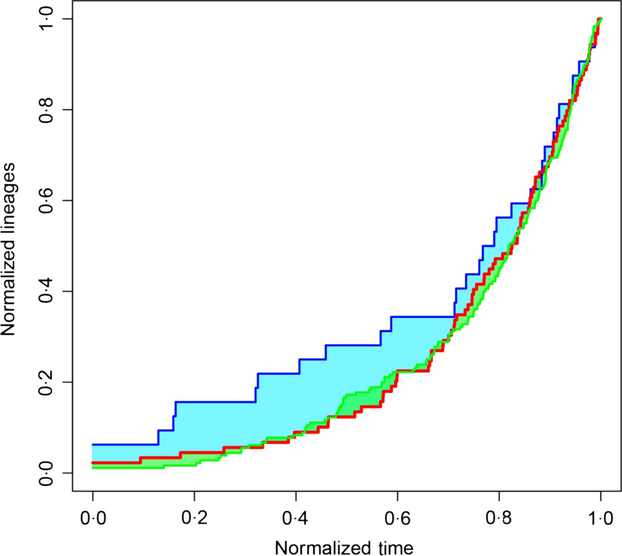
\includegraphics[scale=0.75]{nltt}
  \label{fig:nltt}
\end{figure}

\subsubsection{Adaptive sequential Monte-Carlo approximate Bayseian computation}

I implemented the adaptive sequential Monte-Carlo algorithm
developed in~\autocite{del2012adaptive} for approximate Bayesian computation.
In contrast to most existing sequential Monte-Carlo methods, this algorithm
does not require the user to specify a sequence of decreasing tolerances to
approach the target posterior distribution. Rather, the tolerances are computed
adaptively at each step, starting from infinity at the first iteration. The
algorithm may be stopped when the tolerance reaches a user-defined final value,
or when the rate of acceptance of the MCMC kernel reaches a user-defined
threshold. Following a heuristic applied by the
authors~\autocite{del2012adaptive}, we used the latter stopping criterion,
accepting the SMC approximation to the posterior when the MCMC acceptance rate
dropped below 1.5\%.

\subsection{Method validation}

\subsubsection{Identification of separable parameters in kernel space}
\label{subsubsec:kernel}

\subsubsection{Grid search}

\subsubsection{Approximate Bayesian computation}

\subsection{Applications}

\subsubsection{HIV in British Columubia}
